\chapter{Solver Verification}
\label{ch:verification}

Before applying the solver to the dipole field, it is tested against cases
where the analytic answer is already known. The tests follow a natural
progression: gyromotion in a uniform field, helical motion, drifts in
non-uniform fields, and finally dipole field checks. Each test isolates one
physical effect so that any discrepancy has a clear source.

\section{Circular Gyromotion in a Uniform Field}
\label{sec:test01}

A particle with charge $q=1$, mass $m=1$ is placed at the origin with
velocity $\mathbf{v}_0 = (1,0,0)$ in a uniform field
$\mathbf{B} = \hat{\mathbf{z}}$ and $\mathbf{E} = \mathbf{0}$. Under
these conditions the particle gyrates in the $x$--$y$ plane with Larmor
radius $\rho = v_\perp / \Omega = 1$ and gyroperiod $T_\Omega = 2\pi$.
The guiding centre remains fixed at $(0, -1, 0)$.

Figure~\ref{fig:test01} overlays the numerical orbit with the analytic
circle of radius $\rho = 1$. The two are indistinguishable on this scale:
the maximum radial deviation stays below $10^{-8}$ over 20 time units,
confirming that the solver correctly implements the Lorentz force.

\begin{figure}[htbp]
  \centering
  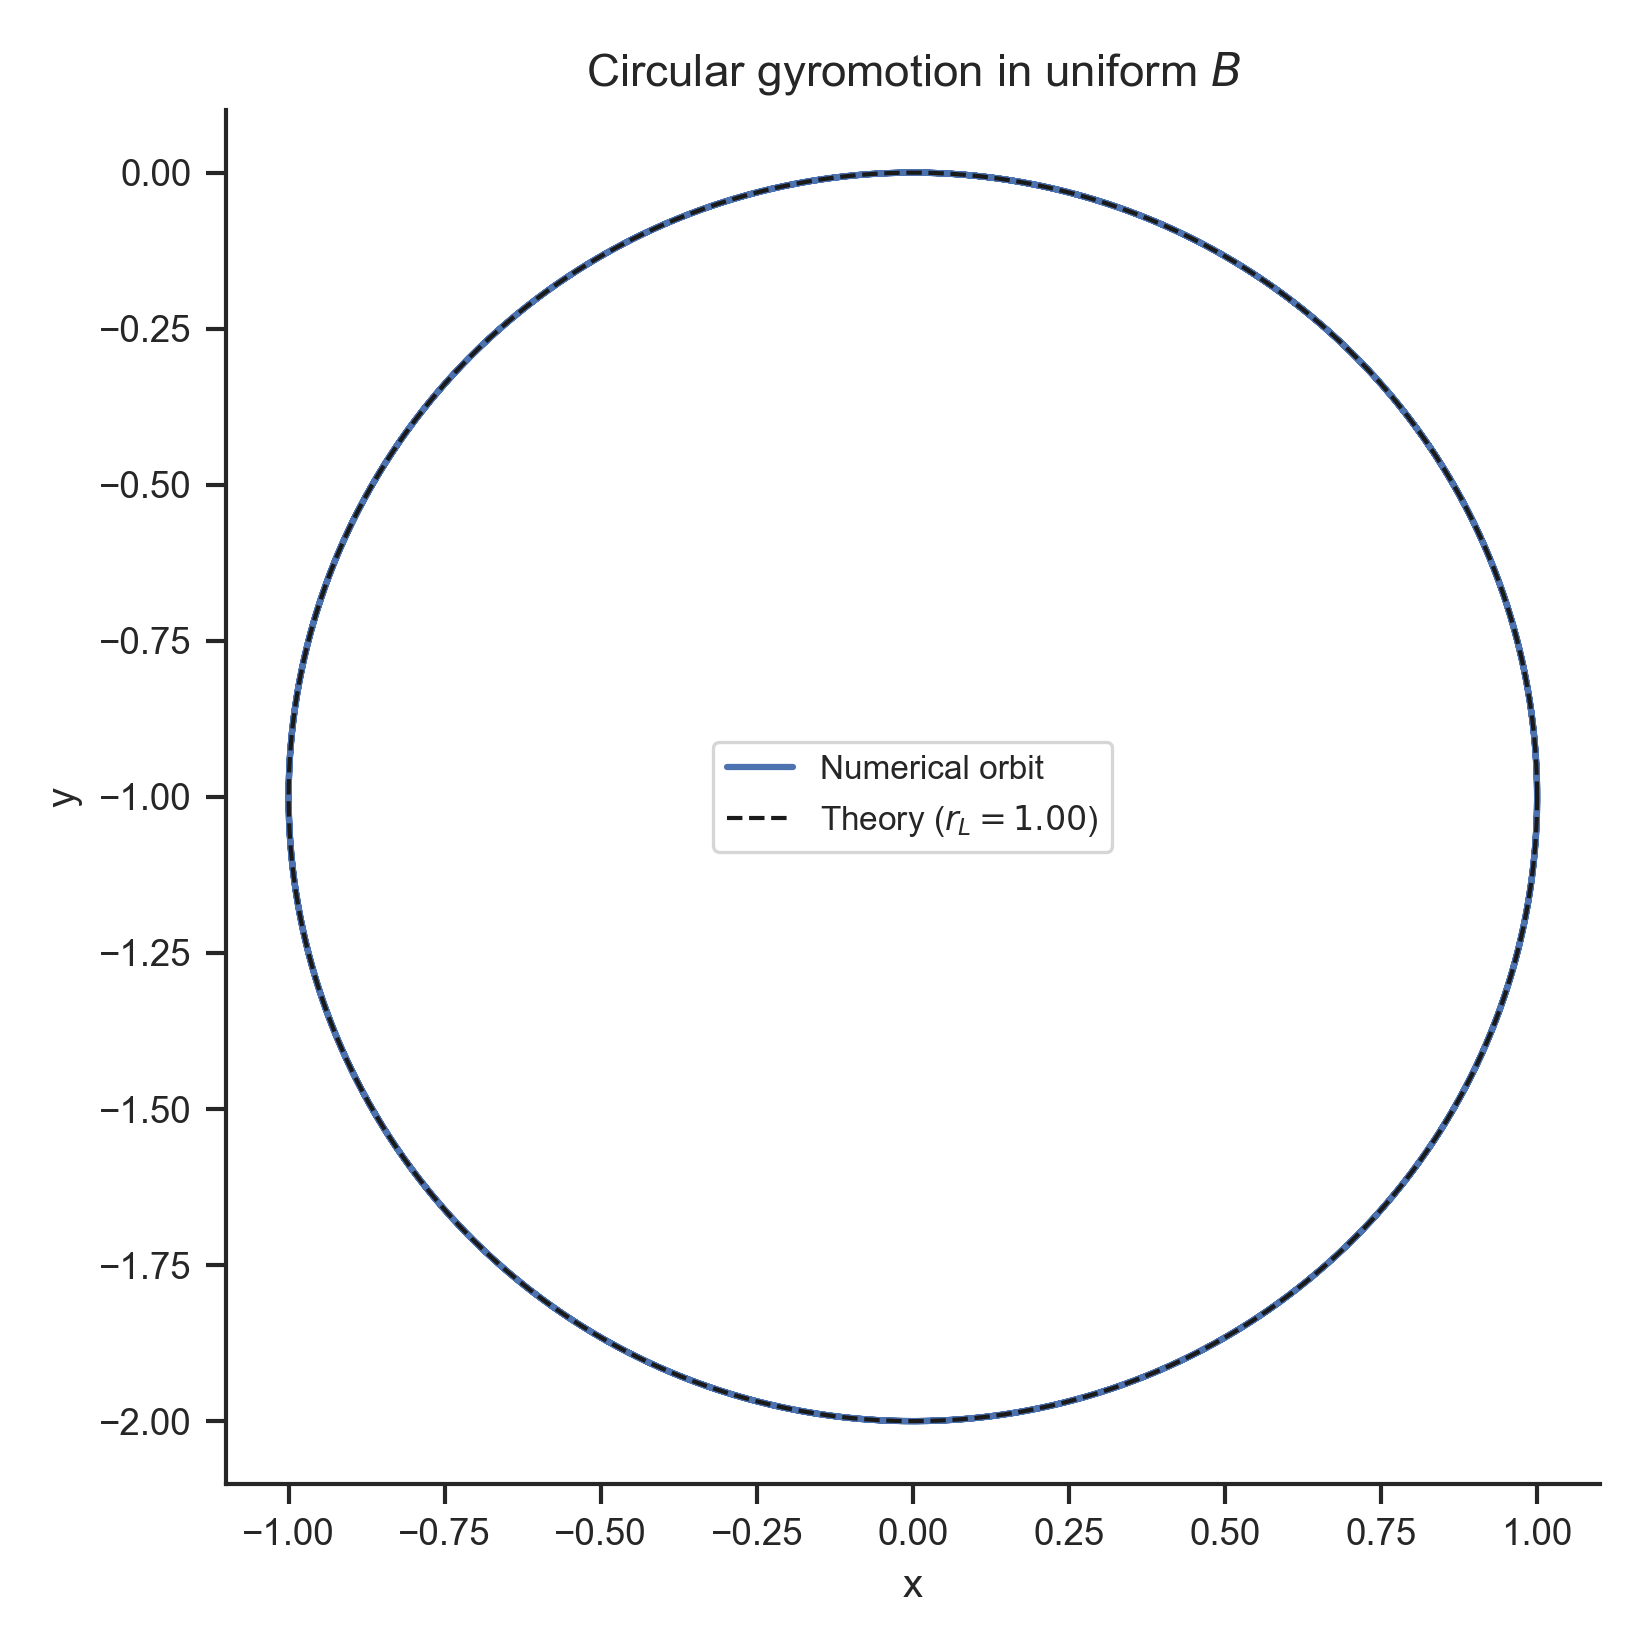
\includegraphics[width=0.5\textwidth]{Figures/test01_uniformB_xy.png}
  \caption{Numerical orbit (solid) and analytic circle of radius $\rho = 1$
    (dashed) in the $x$--$y$ plane. The two curves overlap to plotting
    accuracy.}
  \label{fig:test01}
\end{figure}

\section{Helical Motion}
\label{sec:test02}

Adding a parallel velocity component $v_\parallel = 0.2$ to the same
uniform field gives $\mathbf{v}_0 = (1, 0, 0.2)$. The $x$--$y$ projection
remains a circle of the same Larmor radius, while $z(t) = v_\parallel t$
increases linearly, producing a helical trajectory.

Figure~\ref{fig:test02} shows the resulting 3D helix. The maximum deviation
$|z_\mathrm{num}(t) - v_\parallel t|$ stays below $10^{-9}$ across the full
integration, confirming that parallel and perpendicular motion decouple
correctly in a uniform field.

\begin{figure}[htbp]
  \centering
  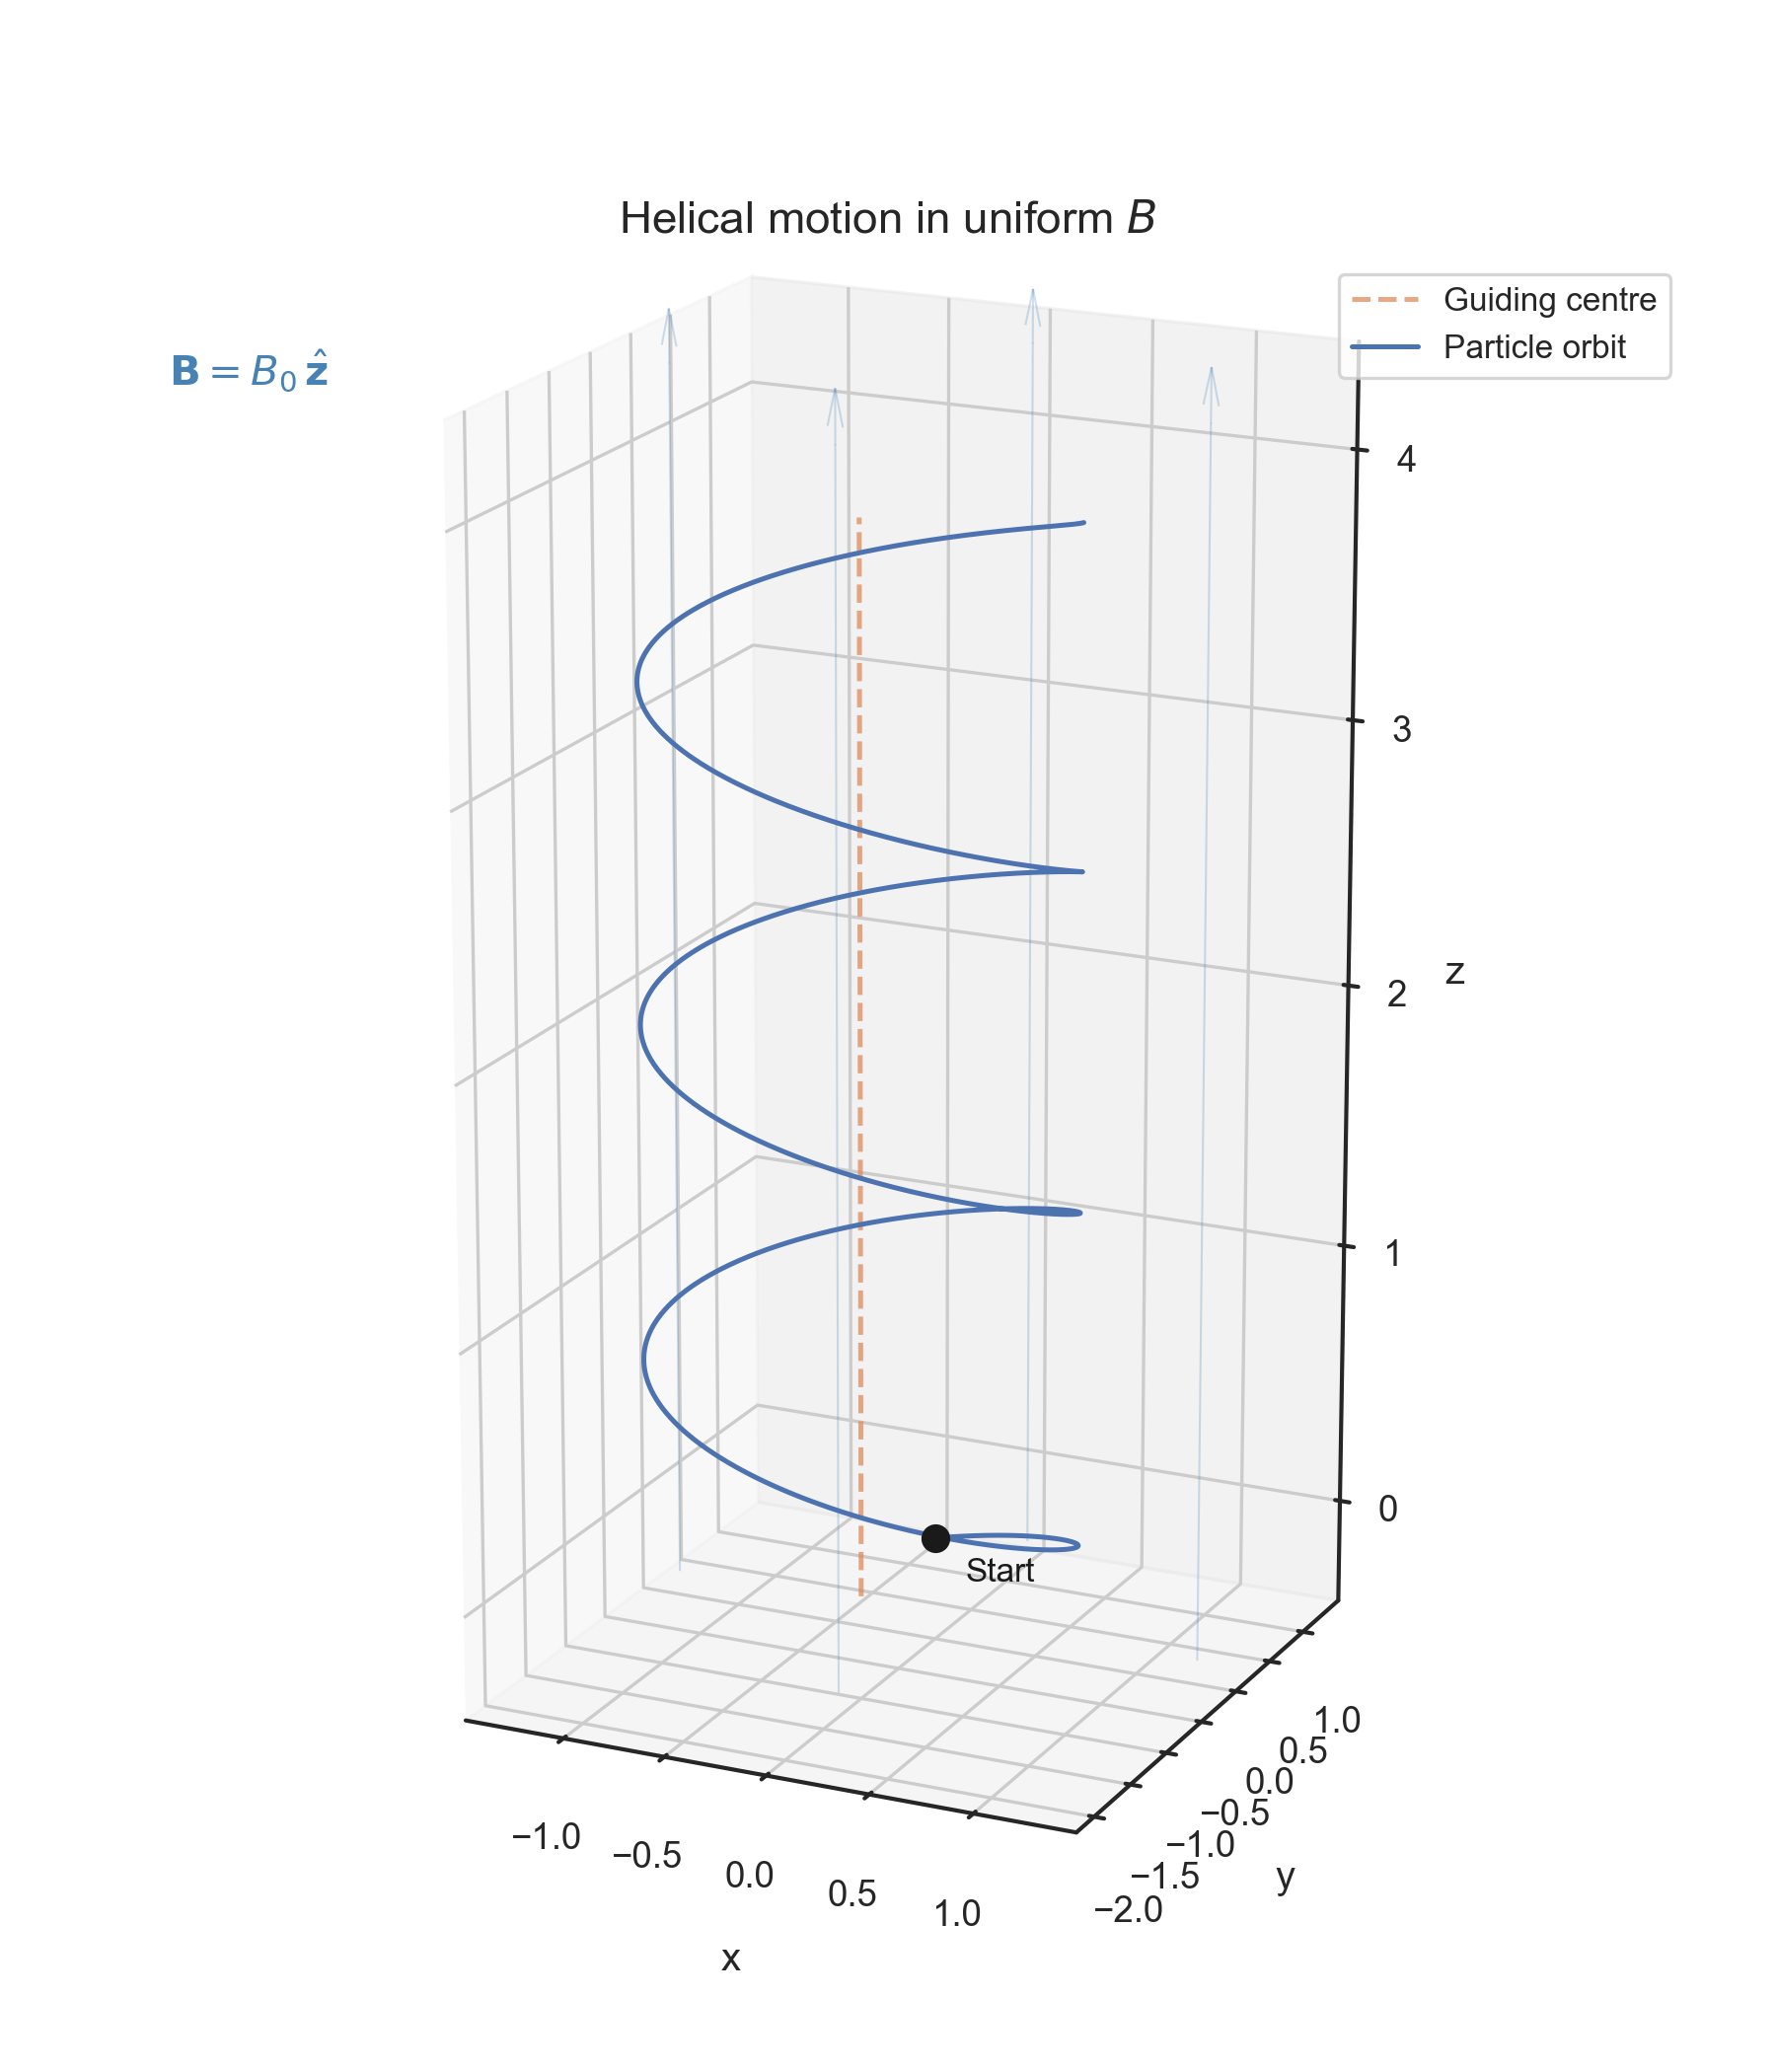
\includegraphics[width=0.55\textwidth]{Figures/test02_uniformB_helix_3D.png}
  \caption{Helical trajectory in a uniform magnetic field. The guiding centre
    advances at constant $v_\parallel = 0.2$ along the field while the
    particle gyrates around it.}
  \label{fig:test02}
\end{figure}

\section{\texorpdfstring{$\mathbf{E}\times\mathbf{B}$}{E x B} Drift}
\label{sec:test03}

With $\mathbf{B} = \hat{\mathbf{z}}$ and a perpendicular electric field
$\mathbf{E} = 0.1\,\hat{\mathbf{x}}$, the guiding centre should drift at
$\mathbf{v}_E = \mathbf{E}\times\mathbf{B}/B^2 = -0.1\,\hat{\mathbf{y}}$,
independent of the particle's charge and mass. The initial velocity is
$\mathbf{v}_0 = (1, 0, 0.2)$ and the integration runs for $T = 50$.

Figure~\ref{fig:test03} shows the $x$--$y$ projection. With $\mathbf{E} = 0$
the orbit is a closed circle; with $E_0 = 0.1$ it becomes a cycloid drifting
in $-\hat{\mathbf{y}}$. A linear fit to the gyro-averaged position gives a
measured drift speed of $-0.1000$ to four significant figures, matching
theory exactly.

\begin{figure}[htbp]
  \centering
  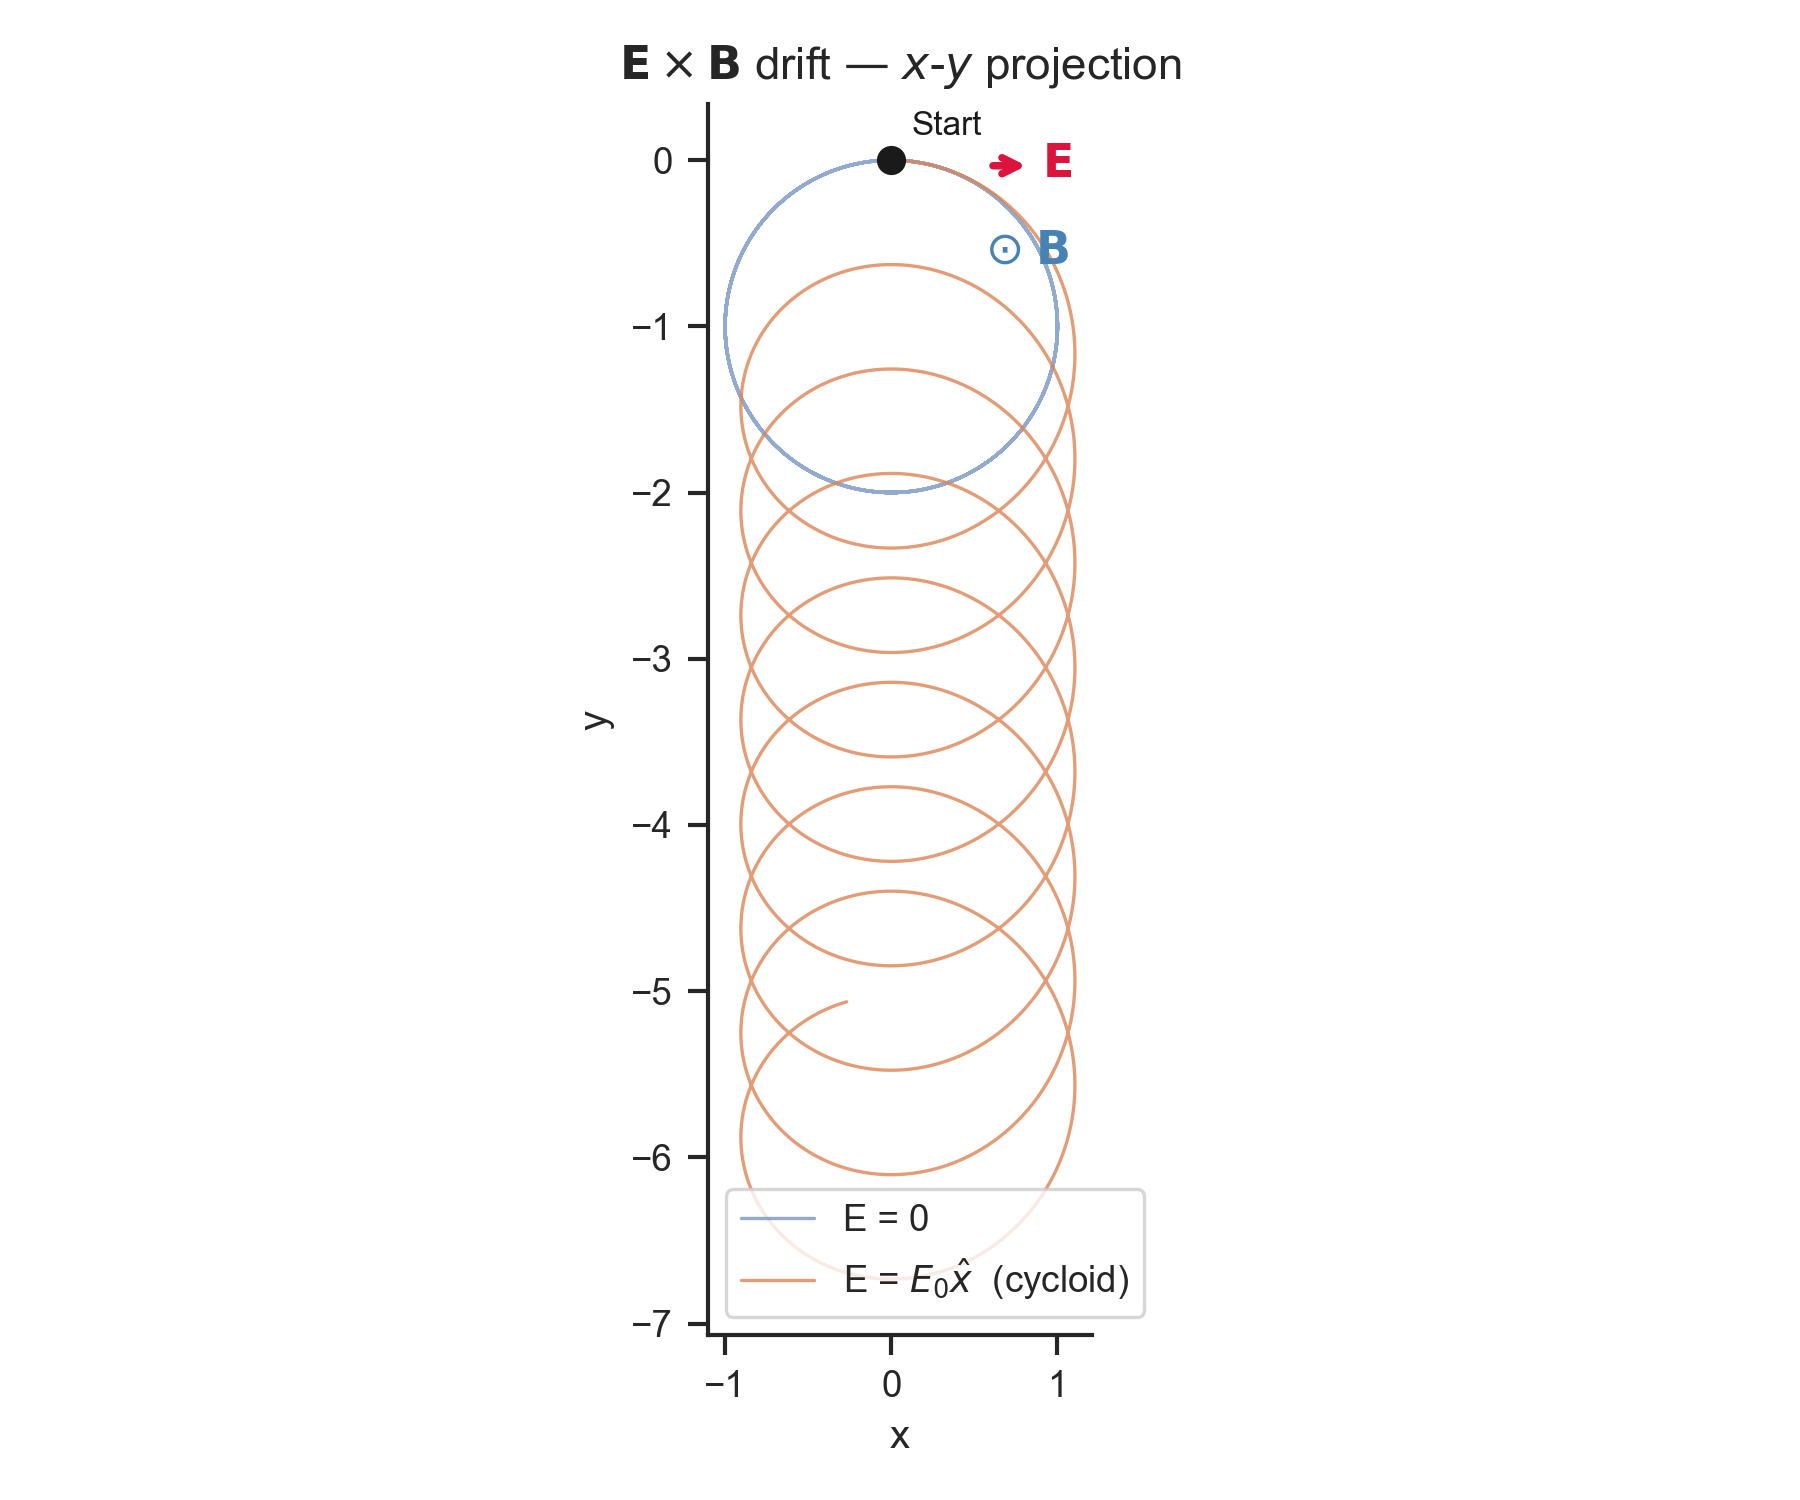
\includegraphics[width=0.55\textwidth]{Figures/test03_exb_xy_projection.png}
  \caption{$x$--$y$ projection showing a stationary circular orbit
    ($\mathbf{E} = 0$, blue) and the cycloid orbit with $\mathbf{E} \times
    \mathbf{B}$ drift ($E_0 = 0.1$, orange). The guiding centre drifts at
    $v_y = -0.1$ in agreement with theory.}
  \label{fig:test03}
\end{figure}

\section{Gradient-\texorpdfstring{$B$}{B} Drift}
\label{sec:test04}

When the magnetic field strength varies in space, the gyroradius is slightly
larger on the weak-field side of the orbit and smaller on the strong-field
side, producing a net drift perpendicular to both $\mathbf{B}$ and
$\nabla|\mathbf{B}|$. To isolate this effect, a field
$\mathbf{B} = B_0(1 + \varepsilon x)\,\hat{\mathbf{z}}$ is used with
$B_0 = 1$, $\varepsilon = 0.05$, and $\mathbf{E} = \mathbf{0}$. This field
has straight field lines, so there is no curvature drift and the
gradient-$B$ contribution can be tested on its own. In a realistic dipole
field, gradient and curvature drifts act simultaneously and cannot be
separated.

The particle starts with $\mathbf{v}_0 = (1, 0.3, 0)$ and is integrated for
$T = 80$. The expected drift speed is
$v_{\nabla B} \approx m v_\perp^2 \varepsilon / (2qB_0)$
(equation~\eqref{eq:gradb_test}).

Figure~\ref{fig:test04} shows the full orbit and extracted guiding centre
in the $x$--$y$ plane. The vertical field lines are spaced inversely with
$|\mathbf{B}|$, visualising the gradient: the Larmor radius is larger on
the weak-field (left) side than on the strong-field (right) side, producing
a net drift in the $-y$ direction. The numerical drift speed agrees with
the analytic value to within 3\,\%, consistent with higher-order
corrections to the first-order drift formula.

\begin{figure}[htbp]
  \centering
  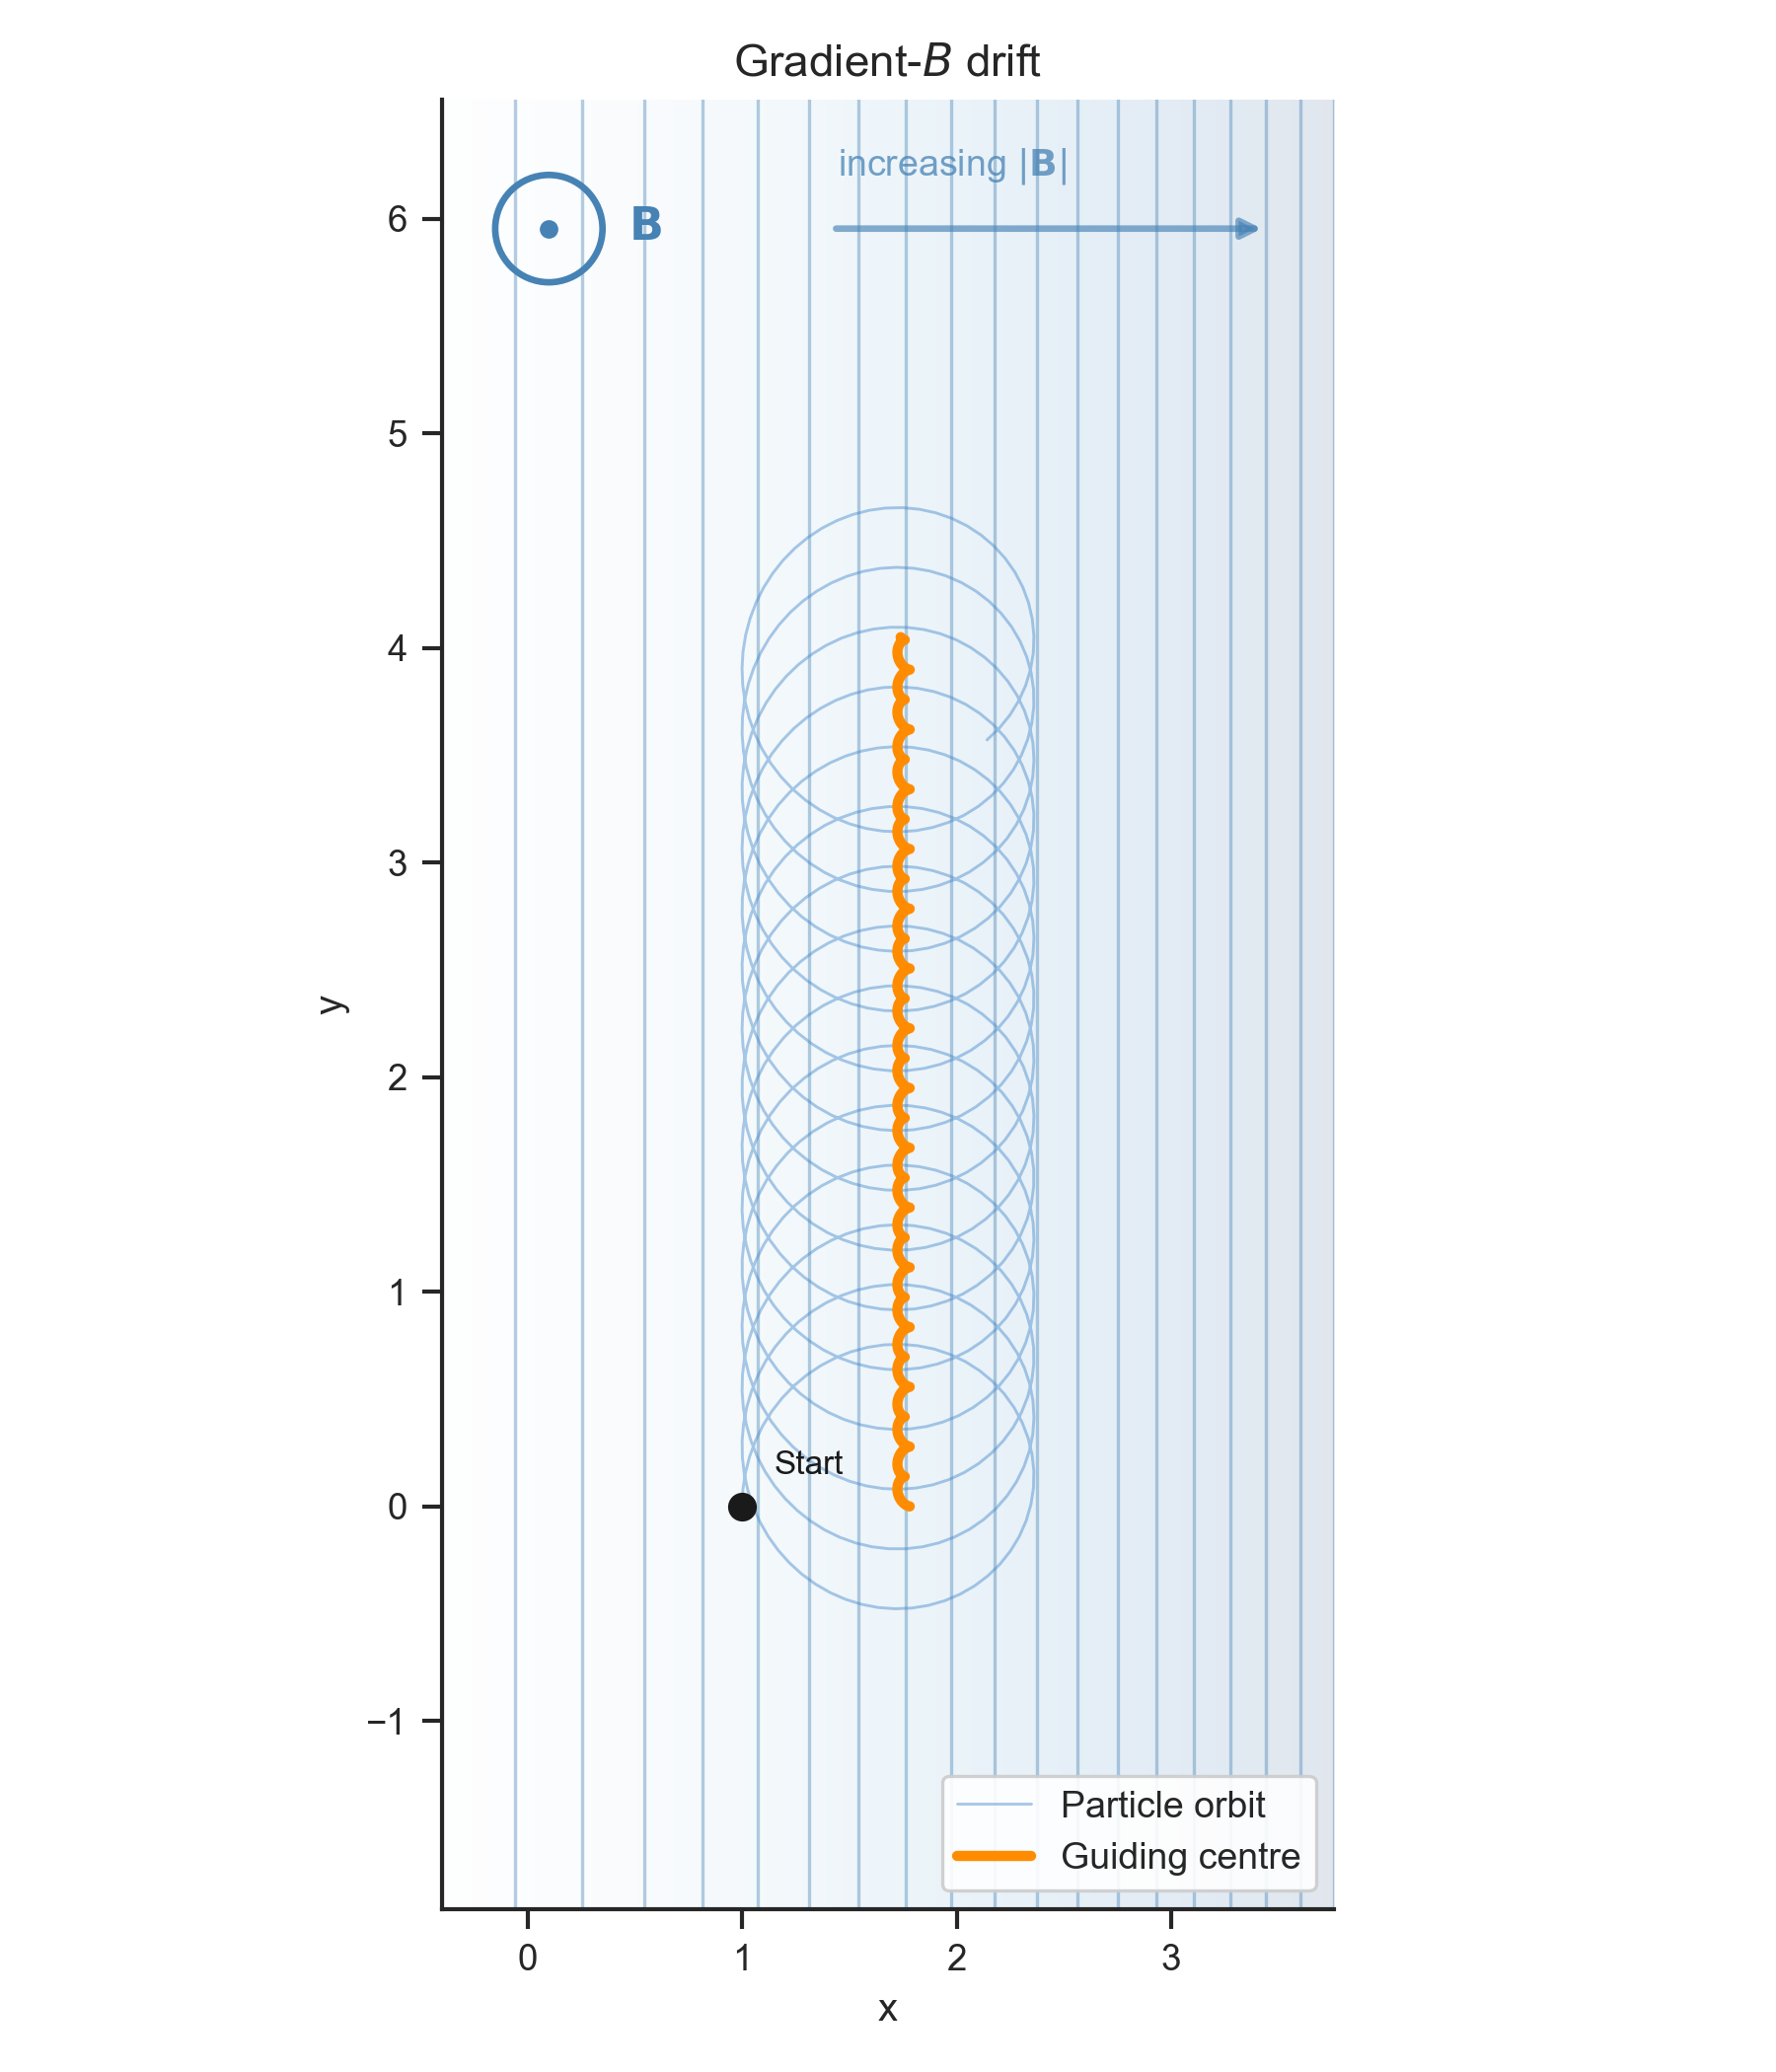
\includegraphics[width=0.55\textwidth]{Figures/test04_gradB_drift.png}
  \caption{Gradient-$B$ drift. Field lines (vertical) are spaced inversely
    with $|\mathbf{B}|$ --- closer together where the field is stronger.
    The particle orbit (blue) shows asymmetric loops; the guiding centre
    (orange) drifts in $-y$.}
  \label{fig:test04}
\end{figure}

\section{Dipole Field Checks}
\label{sec:test07}

Before using the dipole field for orbit simulations, two checks confirm that
the Cartesian expression~\eqref{eq:dipole} is implemented correctly.

Figure~\ref{fig:test07_axis} shows the numerically computed
$|\mathbf{B}(0,0,z)|$ against the analytic formula $2M/z^3$ on logarithmic
axes. The slope matches $-3$ to within $10^{-10}$, confirming the correct
$r^{-3}$ on-axis scaling. Figure~\ref{fig:test07_quiver} shows the field
directions in the $x$--$z$ plane, coloured by $\log_{10}|\mathbf{B}|$. The
characteristic dipole topology is reproduced correctly.

\begin{figure}[htbp]
  \centering
  \begin{subfigure}[b]{0.46\textwidth}
    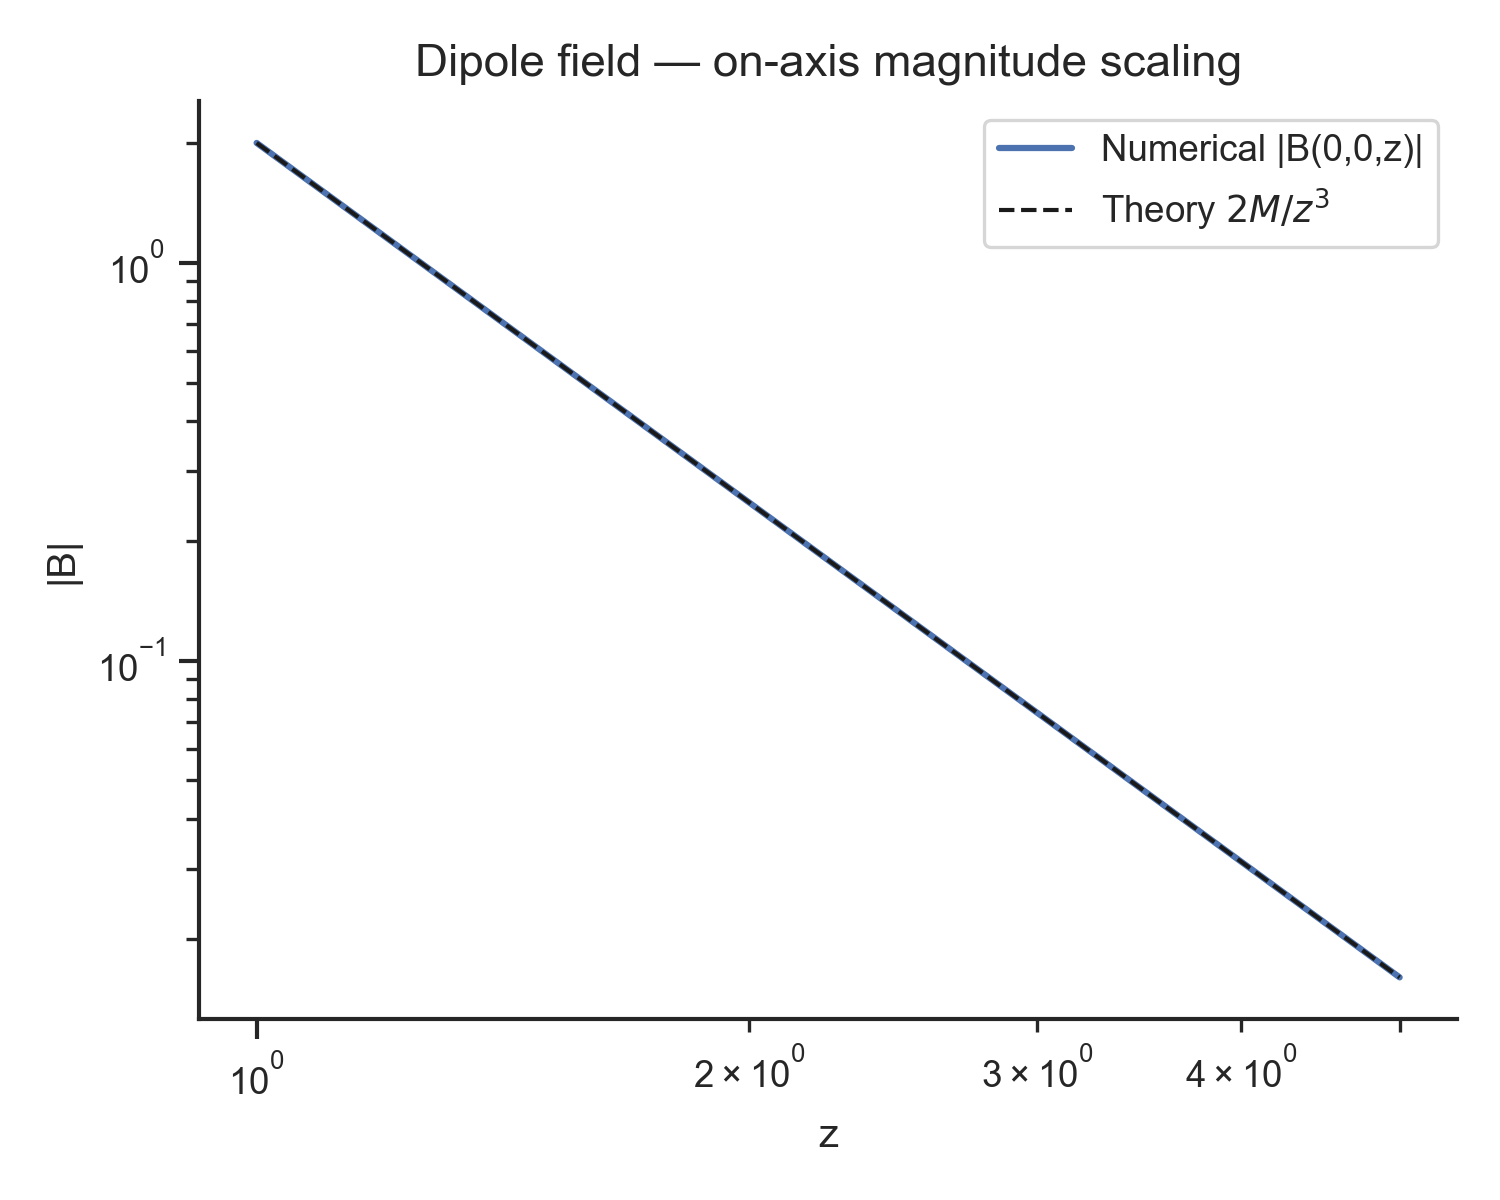
\includegraphics[width=\textwidth]{Figures/test07_dipole_axis_scaling.png}
    \caption{On-axis $|\mathbf{B}|$ vs $z$ (log--log); slope $= -3$.}
    \label{fig:test07_axis}
  \end{subfigure}
  \hfill
  \begin{subfigure}[b]{0.50\textwidth}
    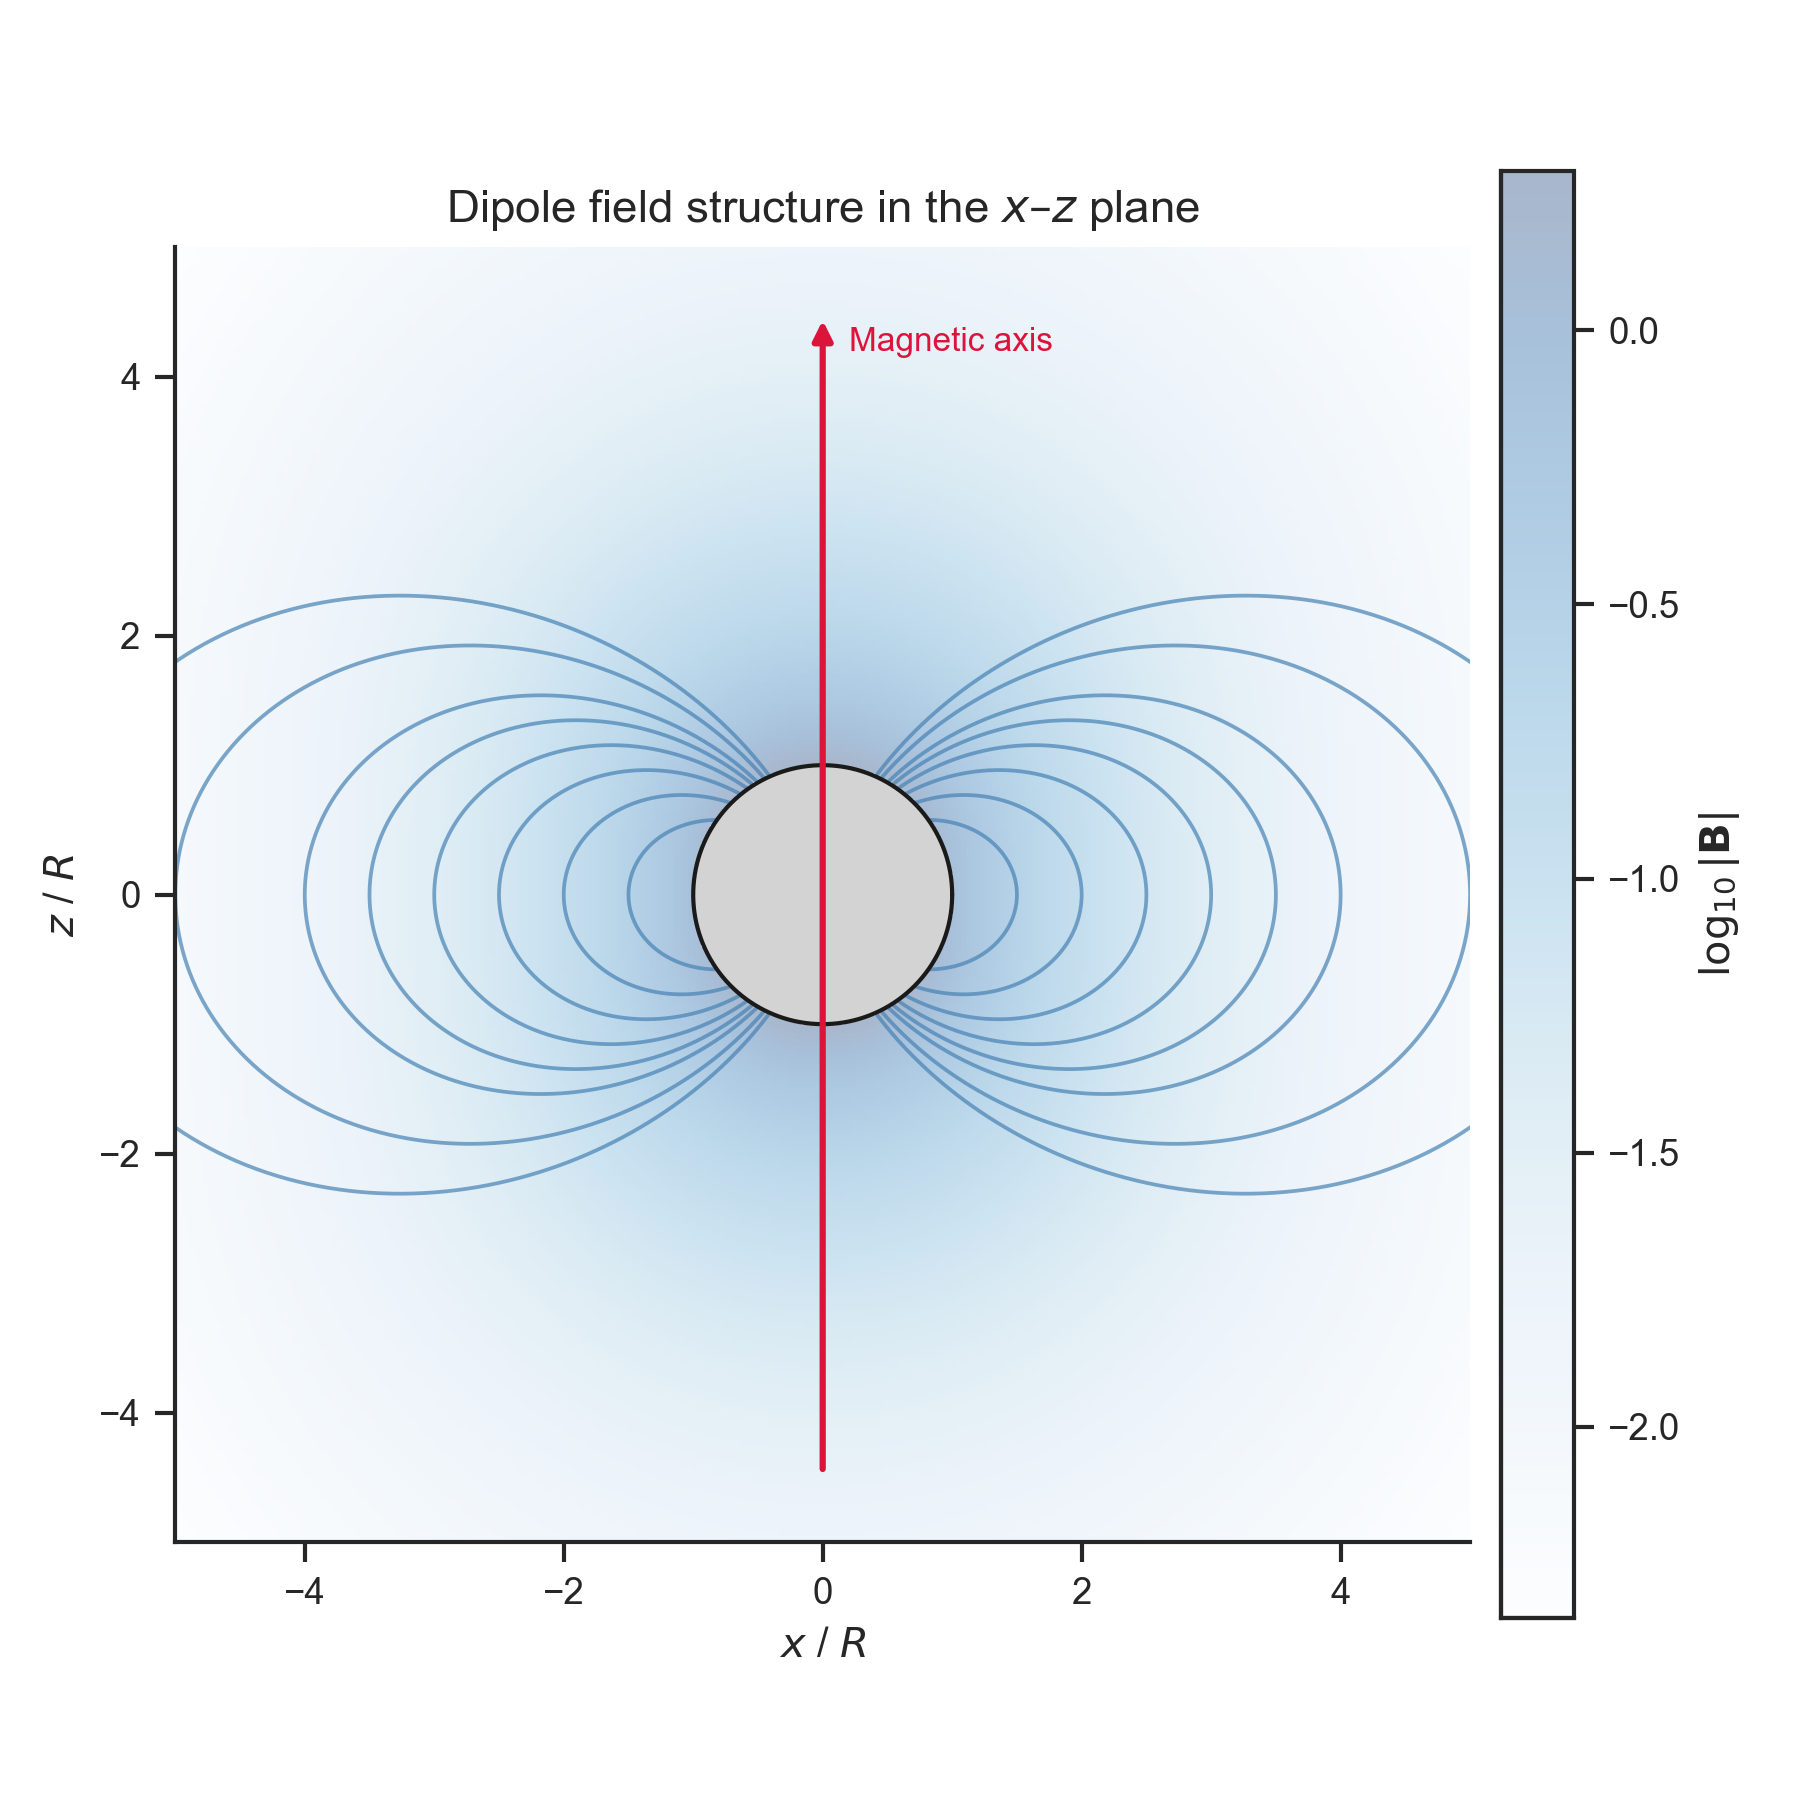
\includegraphics[width=\textwidth]{Figures/test07_dipole_quiver_xz.png}
    \caption{Field directions in the $x$--$z$ plane, coloured by
      $\log_{10}|\mathbf{B}|$.}
    \label{fig:test07_quiver}
  \end{subfigure}
  \caption{Dipole field implementation checks. The on-axis scaling and field
    topology both match the expected dipole structure.}
  \label{fig:test07}
\end{figure}

\section{Energy Conservation}
\label{sec:energy_cons}

For every test with $\mathbf{E} = \mathbf{0}$, the relative kinetic energy
drift $\delta K(t)$ defined in equation~\eqref{eq:energy_diag} stays below
$10^{-6}$ throughout. This confirms that the solver tolerances
(equation~\eqref{eq:tolerances_num}) are appropriate for all simulations in
this project.
